\documentclass[10pt,journal,compsoc]{joser13}
\usepackage[pdftex]{graphicx}
\usepackage{epsfig}
\usepackage{amsfonts}
\usepackage{amsmath}
\usepackage{amsthm}
\usepackage{amssymb}
\usepackage[square,numbers]{natbib}
\usepackage{acronym}
\usepackage{dsfont}
\usepackage{pifont} % http://www.imsc.res.in/Computer/symbols-letter.pdf
\usepackage[pdftex]{thumbpdf}
\usepackage{multirow} % Prevent page breaks occurring within multi-line eqs.
\usepackage{rotating} % text rotation
\usepackage{booktabs} % rules in tables
% \usepackage{array} % alignment of cells in tables
\usepackage{calc}
\usepackage{verbatim}
\usepackage{units}
\usepackage{minted}
\usepackage{float} % separate pages for colour images
\usepackage{color}
% http://www.poeschko.com/2012/01/highlighting-changes-in-latex/
\usepackage{xcolor}
\usepackage[normalem]{ulem}
% \usepackage{trfsigns} % trfsigns.pdf
\usepackage{txfonts} % txfontsdoc.pdf
\usepackage{tikz}
\usepackage{pgfplots}
\usepackage{xmpincl}
\usepackage{eso-pic} % DRAFT
\usepackage{attachfile}

\definecolor{esored}{rgb}{1.00,0.95,0.95}
% http://de.narkive.com/2003/11/26/744404-wasserzeichen-mit-pdflatex.html
\AddToShipoutPicture{
  \put(0,0){
    \resizebox*{!}{\paperheight}{\rotatebox{57}{\hspace{1em}\textcolor{esored}{DRAFT}\hspace{1em}}}}}

% \usemintedstyle{trac}
\usemintedstyle{borland}
% \usemintedstyle{bw}

\definecolor{codegray}{rgb}{0.3,0.3,0.3}
\newcommand{\code}[1]{``\texttt{\textbf{\textcolor{codegray}{\small{#1}}}}''}

\newcommand{\sct}[1]{Section~\ref{cha:#1}}
\newcommand{\equ}[1]{Equation~\ref{equ:#1}}
\newcommand{\anx}[1]{Appendix~\ref{cha:#1}}
\newcommand{\fig}[1]{Figure~\ref{fig:#1}}
% \newcommand{\plt}[1]{Figure~\ref{fig:#1}}
\newcommand{\tbl}[1]{Table~\ref{tbl:#1}}
\newcommand{\lst}[1]{Listing~\ref{lst:#1}}

\acrodef{DSL}{domain specific language}
\acrodef{IRB}{Interactive Ruby Shell}
\acrodef{LOC}{lines of code}
\acrodef{MRI}{Matz's Ruby Interpreter}
\acrodef{REPL}{read-eval-print loop}

%%%%%%%%%%%%%%%%%%%%%%%%%%%%%%%%%%%%%%%%%%%%%%%%%%%%%%%%%%%%%%%%%%%%%%%
%%%%%%%%%%%%%%%%%%%%%%% will be inserted by the editor %%%%%%%%%%%%%%%%
%%%%%%%%%%%%%%%%%%%%%%%%%%%%%%%%%%%%%%%%%%%%%%%%%%%%%%%%%%%%%%%%%%%%%%%
\journalnumber{1}                       %will be inserted by the editor
\journalvolume{1}                       %will be inserted by the editor
\journalmonth{September}                %will be inserted by the editor
\journalyear{2009}                      %will be inserted by the editor
\articlefirstpage{123}                  %will be inserted by the editor
\articlelastpage{126}                   %will be inserted by the editor
\setcounter{page}{123}                  %will be inserted by the editor
%%%%%%%%%%%%%%%%%%%%%%%%%%%%%%%%%%%%%%%%%%%%%%%%%%%%%%%%%%%%%%%%%%%%%%%

\copyrightauthor{J. Wedekind, G. Chliveros, B. P. Amavasai}
\headoddname{J. WEDEKIND et al. / Computer Vision and Device Control using the Ruby Programming Language}

% correct bad hyphenation here
\hyphenation{op-tical
  net-works
  semi-conduc-tor}

\begin{document}
% paper title
\title{Computer Vision and Device Control\\\vskip 0.3\baselineskip using the Ruby Programming Language}

\author{
Jan Wedekind$^{1}$
\qquad
Georgios Chliveros$^{2}$
\qquad
Balasundram P. Amavasai$^{3}$

%%%%%%%%%%%%%%%%%%%%%%%%%%%%%%%%%%%%%%%%%%%%%%%%%%%%%%%%%%%%%%%%%%%%%%%
%%%%%%%%%%%%%%%%%%%%%%% will be inserted by the editor %%%%%%%%%%%%%%%%
%%%%%%%%%%%%%%%%%%%%%%%%%%%%%%%%%%%%%%%%%%%%%%%%%%%%%%%%%%%%%%%%%%%%%%%
\thanks{{\bf Regular paper} -- Manuscript received April 19, 2009;
revised July 11, 2009.}
%%%%%%%%%%%%%%%%%%%%%%%%%%%%%%%%%%%%%%%%%%%%%%%%%%%%%%%%%%%%%%%%%%%%%%%

\IEEEcompsocitemizethanks{\IEEEcompsocthanksitem This work was partially funded
  by the EPSRC Nanorobotics grant and a student bursary by the Materials and
  Engineering Research Institute at Sheffield Hallam University.\protect\\

  \IEEEcompsocthanksitem Authors retain copyright to their papers
  and grant JOSER unlimited rights to publish the paper electronically and in
  hard copy. Use of the article is permitted as long as the author(s) and the
  journal are properly acknowledged.}

} % end author

\address{
$^1$ 7 William Road, Sutton SM1 4QT, United Kingdom\\
$^2$ Institute of Computer Science, Foundation for Reasearch and
Technology - Hellas, Heraklion, Crete, Greece\\
$^3$ 96 Brooksby Road, Reading R31 6LY, United Kingdom}

% The paper headers
\markboth

\IEEEcompsoctitleabstractindextext{%
% No more than 500 words
% define all nonstandard symbols and acronyms used
\begin{abstract}
  $\ldots$
\end{abstract}

\acresetall % repeat definitions even if introduced in abstract already

% 2-5 keywords from http://www.old.ieee-ras.org/uploads/tro/T-RO_Keywords.pdf
% or http://www.computer.org/portal/web/publications/acmtaxonomy
\begin{IEEEkeywords}
  Computer Vision,
  Image processing software,
  Input/output,
  Interactive systems,
  Reusable libraries,
  Very high-level languages.
\end{IEEEkeywords}}


% make the title area
\maketitle

% MISLA

\section{Introduction}
% The very first letter is a 2 line initial drop letter followed
% by the rest of the first word in caps.
\IEEEPARstart{M}{achine} vision is an important part of the interdisciplinary
field of robotics. Developers of programming systems in general and machine
vision software in particular face the challenge of bringing together
\begin{itemize}
  \item performance
  \item productivity
  \item generality
\end{itemize}
in a single architecture (see \fig{triangle}).
\begin{figure}[htbp]
   \begin{center}
     \resizebox{.5\columnwidth}{!}{
\includegraphics{triangle}}\\
     \caption{The main requirements when designing a programming language or
     system \citep{wolczko2011}\label{fig:triangle}}
   \end{center}
\end{figure}

Scripting languages offer a great productivity advantage and the productivity
of programmer's measured in \ac{LOC} per hour seems to be independent of the
programming language\citep{prechelt2000empirical}. However performance is
critical when implementing a machine vision system. \emph{I.e.} when
prototyping a machine vision system using a scripting language such as Octave
(productivity \& generality), it is usually necessary to later port it to a
compiled language such as C/C++ (performance \& generality) to implement the
final system.

Today's desktop software is dominated by complex software systems which cannot
be understood by a single person any more. However most of this complexity can
be shown to be "accidental" rather than inherent\citep{ohshima2013kscript}.
Using \acp{DSL}, one can keep the size of software systems (measured in LOC)
\emph{orders of magnitudes} smaller and thus more
manageable\citep{kay2010steps}.

In this paper we are going to show how the Ruby programming language (which has
strong support for DSLs) can help to reduce accidental complexity when
implementing real-time machine vision software.

\section{Ruby Programming Language}
The Ruby programming language\footnote{\url{http://www.ruby-lang.org/}} is an
\emph{interpreted language}. It uses a \emph{mark-and-sweep} garbage collector
for memory management. Important features of the programming language are
\begin{itemize}
  \item \emph{late binding}
  \item \emph{closures}
  \item \emph{exception handling}
  \item \emph{continuations}
  \item \emph{open classes}
\end{itemize}

Ruby has support for \emph{meta-programming}. In particular
\begin{itemize}
  \item \code{methods} returns an object's list of available methods
  \item \code{define\_method} defines a method at runtime
  \item \code{method\_missing} traps calls to nonexistent methods
  \item \code{send} dynamically calls a method
\end{itemize}

\ac{MRI} (the reference implementation of Ruby) comes with tool called the
\ac{IRB}. \ac{IRB} is a \ac{REPL} for the Ruby programming language. \lst{repl}
shows an example of an \ac{IRB} session. Comment lines (preceded with \code{\#}) show the output of the interpreter.
\begin{listing}[htbp]
  \begin{minted}[fontsize=\footnotesize]{ruby}
class Test
  def initialize(x)
    @x = x
  end
  def inspect
    "Test(#{@x})"
  end
end
# nil
Test.new 3
# Test(3)
Test.new(3).inspect
# "Test(3)"
  \end{minted}
  \caption{The role of inspect methods when using IRB\label{lst:repl}}
\end{listing}

The \ac{IRB} session shown in \lst{repl} illustrates an important feature of Ruby: After evaluation the interpreter calls the \code{inspect} method of the result in order to display it. \emph{I.e.} the user can control the way an object is displayed by implementing the \code{inspect} method. \fig{object} shows an UML diagram of the class defined in \lst{repl}.
\begin{figure}[htbp]
  \begin{center}
    \resizebox{.6\columnwidth}{!}{\includegraphics{object}}
    \caption{Ruby object with \code{inspect} method\label{fig:object}}
  \end{center}
\end{figure}

\begin{listing}[htbp]
  \begin{minted}[fontsize=\footnotesize]{ruby}
def expect(x, &action)
  while true
    v = action.call
    break if v >= x
  end
  v
end
# nil
a = 1
# 1
expect(5) { a += 3 }
# 7
  \end{minted}
  \caption{Implementing custom control structure using a closure\label{lst:closure}}
\end{listing}
% Closures $\Rightarrow$ custom control structures! (video input)

% Ruby: coerce/numerical library, unit testing,

% empirical evidence for productivity (LOC, structural complexity)
% theoretical contribution: generic operations, more fundamental understanding
% of computer vision

% (Const.new) MRI: single threaded (JRuby?, Rubinius?), meta-programming does
% not cover control statements (while, if, ...)


% No architecture: don't impose a static datatype for representing images etc

% Integration

% JIT compilation (using GCC): fetch, construct, store, coerce, coercion,
% descriptor, dup, compilable?, strip, get, assign, write, storage\_size,
% memory\_type, default, inspect

% fast development cycle

% maximally generic (binary operations (no subset of integer types),
% histograms, tensor operations, luts/warps, map (unary operation), inject,
% mask/unmask (larrabee), integral, convolution)

% Possible topics for papers submitted to the journal include but
% are not limited to:
% \begin{itemize}
%     \item Analysis of issues and challenges in the development of robot
%     software systems, that make the robotic domain similar/different to other
%     application domains (e.g. automotive, factory automation)
%     \item Identification of recurrent concepts, aspects, and requirements in
%     robot software systems, that may lead to the definition of standard /
%     common / unified specifications, design models, interfaces, protocols,
%     and software libraries
%     \item Documentation of measures and procedures to evaluate software
%     quality factors
%     \item Description of conceptual tools as well as software environments
%     that simplify the design, implementation, and reuse of robot software
%     systems.
%     \item Exploitation of software engineering conceptual tools (e.g. formal
%     specification and verification methods) to cope with specific robotic
%     requirements (e.g. fault tolerance, robustness, autonomy, real-time
%     guarantee)
%     \item Experience reports and case studies of successful development of
%     software systems for real robotic applications.
% \end{itemize}
%
% These instructions give you guidelines for preparing papers for
% JOSER. Download the LaTeX template files from the website
% \url{http://www.joser.org/public/download/josertex.zip} so you can use the
% templates to prepare your manuscript.

% \section{Editorial Policies}
% This journal provides immediate open access to its content on the
% principle that making research freely available to the public
% supports a greater global exchange of knowledge.
% Papers will be available on the JOSER Web portal as soon as they have been
% approved by the reviewers.
%
% \subsection{Type of papers}
% Submitted articles may be of three basic types:
%
% {\bf Regular papers}: Detailed discussion involving new
% research, applications or developments. There is no length limit
% on regular papers. The nominal length is 10 single-spaced, double
% column pages including figures and bibliography. However, it is
% recommended that papers not exceed 15 single-spaced, double column
% pages. Papers that exceed this recommended maximum length will
% still be considered, but might not be guaranteed editorial review
% or publication in a timely fashion.
%
% {\bf Short papers}: Brief presentations of new technical concepts
% and developments. Short papers should not exceed 6 single-spaced
% double column pages including figures and bibliography.
%
% {\bf Comments}: Comments are brief contributions that comment on
% previously published papers. These may include reports on
%
% \begin{itemize}
%     \item exploitation and validation of research results
%     \item interpretation of experimental data
%     \item opinions about open issues
% \end{itemize}
% Comments should equal 4 single-spaced double column pages (including
% reasonably sized figures and references).


%\subsection{Review criteria}
%Papers are reviewed and evaluated according to the following criteria.
%\begin{itemize}
%    \item Relevance. Descriptions of pure sensor processing, planning or
%    control get a lower score than documentations of (1) software
%    architectures that help to integrate these core aspects of robotics, (2)
%    software requirements that have been taken into account (portability,
%    reusability, maintainability, interoperability, etc.), (3) metrics and
%    methods that allow to assess software quality factors of robotic systems,
%    or (4) computational issues related to the implementation of robotics
%    algorithms. Papers should report on what was learned in doing the work,
%    rather than merely on what was done.
\section{$\ldots$}
\begin{itemize}
  \item Software architecture based on memory objects (Malloc) allows
    integration (no C++ "static" types).
  \item Requirements: generic operators on n-dimensional arrays, high
    performance, binary operations on any element-type (including array),
    generic operators instead of monolithic implementations
  \item Ruby allows for functional testing
  \item Using closures during camera initialisation and for displaying videos
\end{itemize}
%    \item Significance. Descriptions of ad-hoc software library, framework, or
%    middleware for specific robotic systems get a lower score that
%    documentation of reuse/adaptation/reengineering of existing software
%    artifacts. When appropriate, authors are encouraged to demonstrate the
%    utility of their work on significant problems; any experiments reported
%    should be     reproducible. Contributions to relevant standards,
%    benchmarks, software patterns as well as their adoption in novel
%    application contexts are positively evaluated.
\begin{itemize}
  \item Integration of existing I/O libraries: ALSA, DC1394, FFMpeg, Kinect,
    OpenEXR, Qt4, RMagick, V4L2, Xorg
  \item Integration with other libraries: FFTW3, libswscale, linalg, narray,
    opencv
  \item Utility of the work: TODO
\end{itemize}

\section{$\ldots$}

\section{Conclusion}
% Typical functions of the conclusion of a scientific paper include 1)
% summing up, 2) a statement of conclusions, 3) a statement of
% recommendations, and 4) a graceful termination. Any one of these, or
% any combination, may be appropriate for a particular paper. Some
% papers do not need a separate concluding section, particularly if
% the conclusions have already been stated in the introduction.
Racket, Clojure, Factor, STEPS project

%    \item Originality. The work cannot have been published previously or be
%    pending publication in another journal, and submissions cannot be under
%    review or be sent for review in any other journal. We will consider
%    research that has been published, or is under consideration for
%    publication at workshops or conferences. In these cases, we expect the
%    JMLR submission to go into greater depth and extend the published results
%    in a substantive way. Authors must notify JOSER about previous or pending
%    conference publication at the time of submission.
%    \item Technical quality. Use of standard modeling languages (e.g. UML,
%    SysML, Marte, AADL) is positively evaluated as well as motivation why
%    existing standards are not sufficient for the authors purpose. All
%    claims should be clearly articulated and supported either by empirical
%    experiments or theoretical analyses.
%    \item Presentation. Papers must be concise and complete; manuscripts
%    should be carefully proofread and polished. Submissions that do not meet
%    these criteria may be returned unreviewed.
%\end{itemize}

%\section{Manuscript submission}
%Authors need to register with the journal prior to submitting, or if already
%registered can
%simply log in and begin the 5 step process.
%All submissions are acknowledged.

% An example of a floating table. Note that the
% \caption command should come BEFORE the table. Table text will default to
% \footnotesize.
% The \label must come after \caption.
%
%\begin{table}[!t]
%\renewcommand{\arraystretch}{1.3}
%\caption{An Example of a Table}
%\label{table_example}
%\centering
%\begin{tabular}{|c||c|}
%\hline
%One & Two\\
%\hline
%Three & Four\\
%\hline
%\end{tabular}
%\end{table}

% \subsection{Initial Submission}
% Articles must be submitted in PDF. Submissions should be typeset
% in 11 point font or larger, and should include all author contact
% information on the first page.
%
% Although not required for submission, we encourage authors to use
% the JOSER LaTeX style package (described hereafter).
%
% Articles may be accompanied by online supplemental material.
% (Note: if an online appendix contains source code, we will require
% you to sign a release form prior to publication freeing us from
% liability.)
%
% To submit a paper, please
% \begin{enumerate}
%    \item Prepare it in PDF.
%    \item Ensure that the file to be uploaded is less than 5Mb in size.
%    \item Ensure that the title page contains
%    \begin{itemize}
%           \item complete name, postal and e-mail address of the corresponding
%           author;
%           \item an abstract that does not exceed 500 words
%           \item a list of minimum two keywords (five recommended)
%    \end{itemize}
%    \item Register, log in, and begin the 5 step process.
% \end{enumerate}
%
% \subsection{Camera-ready copies of accepted papers}
% To ensure that all articles published in the journal have a
% uniform appearance, all camera-ready copies of accepted papers are
% required to be typeset in LaTeX with the JOSER LaTeX style
% package.
%
% Camera-ready copies of accepted papers which do not adhere to JOSER author
% guidelines WILL NOT be published. Authors must submit camera-ready papers as
% zip files that include:
% \begin{enumerate}
%     \item a single source file author\_yyyymmdd.tex; do not include external
%     .tex files; use the submission date
%     \item the bibliography file author\_yyyymmdd.bib (only for BibTeX users)
%     \item the collection of figures as jpg or png files
%     author\_yyyymmdd\_f01.jpg, \_f02.jpg, etc.
%     \item the output file author\_yyyymmdd.pdf
% \end{enumerate}
%
% \section{Manuscript preparation}
% Manuscripts should include the following parts: title, authors$'$
% names, authors$'$ affiliations, abstract, keywords, text,
% acknowledgments (if necessary), collected references (e.g.
% ~\cite{IJSEK1996:Stewart, SEER2007:Vaughan, ROBIO2006:Friedmann,
% SIMPAR2008:Petters} and ~\cite{JARS2006:Colon, IJAR2001:Zielinski,
% IEEE-TSE1997:Stewart, ICIAS2008:Spexard,
% IROS2003:Montemerlo}), short
% biography and the photographs of every author (above 600 dpi),
% tables and figures (above 600 dpi). Supplemental material should
% be briefly described in section "Appendixes".
%
% \subsection{Abbreviations and acronyms}
% Define abbreviations and acronyms the first time they are used in
% the text, even after they have already been defined in the abstract
% or keywords. Abbreviations such as IEEE, SI, etc., do not have
% to be defined. Abbreviations that incorporate periods should not
% have spaces: write ``C.N.R.S.,'' not ``C.\ N.\ R.\ S.''
%
%
% \subsection{Figures and tables}
% Please verify that the figures and tables you mention in the text actually
% exist.
%
% Every figure must have a caption that is complete and intelligible
% in itself without reference to the text.
%
% The preferred format is jpg for figures
% with a minimum resolution of 600 dpi (dots per inch).
% The description style of the figures is specified as ``Time New
% Roman 8pt-12pt''. Figures can be in color or grayscale.
%
% \begin{figure}[!t]
% \centering
% 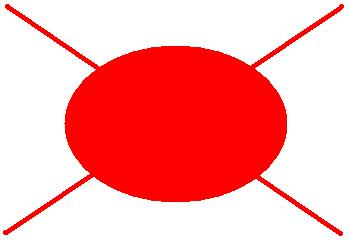
\includegraphics[width=2.5in]{figure}
% \caption{It is good practice to explain the significance
% of the figure in the caption}
% \label{fig:afigure}
% \end{figure}
%
%
% \section*{Supplemental material}
% JOSER accepts supplemental materials for review and publication with regular
% paper submissions.
%
% Types of supplemental material include:
% \begin{itemize}
%     \item proofs
%     \item code
%     \item experimental data
%     \item Graphics should be in JPEG, GIF, PNG, or TIFF format.
%     \item Movies/Animations: .MOV, .AVI, .QT. MPEG files acceptable,
%     QuickTime 3 format preferred, under 4 minutes in length, 320x240 pixels.
%     File size must be minimized and download time must be considered. We
%     recommend files not exceed 30 MB. Files larger than this may be returned
%     for modification to make them smaller.
% \end{itemize}
%
% If you intend to submit supplemental material, please describe it
% shortly in this section.
%
%
\section*{Acknowledgments}
The authors would like to thank...

% references section
\bibliographystyle{IEEEtran}
% argument is your BibTeX string definitions and bibliography database(s)
\bibliography{IEEEabrv,joser13}


% biography section
\begin{IEEEbiography}[{wedekind}]{Jan Wedekind}
received his B.\,Sc. and
M.\,Sc. degrees in mechanical engineering from the *** University,
in 1977 and 1984, respectively, and the Ph.\,D. degree in
computing from *** University, in 1992. In 1994, he was a
faculty member at *** University and in 1996 at ***
University. Currently, he is a professor in the Department of
Information System Engineering at *** University.
He has published about 100 refereed journal and conference papers.
His research interest covers robotics, software engineering, and distributed
systems.
Prof. Author received research award from Science Foundation, and
the Best Paper Award of the XX International Conference in 2000 and
2006, respectively. He is a member of ACM and IEEE.
\end{IEEEbiography}

\begin{IEEEbiography}[{chliveros}]{Georgios Chliveros}
received his PhD in Pattern Recognition from Sheffield Hallam University (SHU)
in 2005. His undergraduate studies were on instrumentation systems and
his postgraduate studies on industrial statistics. 
He was a researcher in robotics at the Materials and Engineering Research Institute, SHU
from 2004 to 2011. Currently he is a research engineer in machine vision and robotics at
the Foundation for Research and Technology Hellas (ICS-FORTH).
His research interests are on robotic systems and
computational engineering methods.
He is a member of the IET, UK and fellow of the RSS, UK.
\end{IEEEbiography}

\begin{IEEEbiography}[{amavasai}]{Balasundram P. Amavasai}
received his B.\,Sc. and
M.\,Sc. degrees in mechanical engineering from the *** University,
in 1977 and 1984, respectively, and the Ph.\,D. degree in
computing from *** University, in 1992. In 1994, he was a
faculty member at *** University and in 1996 at ***
University. Currently, he is a professor in the Department of
Information System Engineering at *** University.
He has published about 100 refereed journal and conference papers.
His research interest covers robotics, software engineering, and distributed
systems.
Prof. Author received research award from Science Foundation, and
the Best Paper Award of the XX International Conference in 2000 and
2006, respectively. He is a member of ACM and IEEE.
\end{IEEEbiography}

% insert where needed to balance the two columns on the last page with
% biographies

% You can push biographies down or up by placing
% a \vfill before or after them. The appropriate
% use of \vfill depends on what kind of text is
% on the last page and whether or not the columns
% are being equalized.

\vfill

% Can be used to pull up biographies so that the bottom of the last one
% is flush with the other column.
%\enlargethispage{-5in}

% that's all folks
\end{document}
